\documentclass[12pt, class=article, crop=false]{standalone}
\usepackage[subpreambles=true]{standalone}
\usepackage[T1]{fontenc} % for font setting
\usepackage{newtxtext,newtxmath}
\usepackage{import,
            graphicx,
            parskip,
            url,
            amsmath,
            wrapfig,
            fancyhdr,
            xcolor}

% for special characters in bibliography            
\usepackage[utf8]{inputenc}
\usepackage[T1]{fontenc}

% citation setup
\usepackage[sort&compress]{natbib}
\setcitestyle{square}
\setcitestyle{comma}

% side caption figure
\usepackage{sidecap}
\sidecaptionvpos{figure}{t}

% caption setup
\usepackage[font={fontenc, small}, labelfont={bf, small}]{caption}

% color box
\usepackage[most]{tcolorbox}

% margin
\usepackage[top=2.54cm, bottom=2.54cm, left=2.54cm, right=2.54cm, marginparwidth=2cm]{geometry}

% header
\pagestyle{fancy}
\fancyhead[L]{Project Narrative}
\fancyhead[R]{}

\tcbuselibrary{breakable}
\bibliographystyle{pnas-new}
\graphicspath{{output/}}

\begin{document}

\newtcolorbox{roundbox}{
  colback=white,
  colframe=gray,
  coltext=black,
  parbox=false,
  boxsep=5pt,
  arc=1pt}

\section{Introduction}

\subsection{Overview}

Freshwater ecosystems provide ecosystem services essential to humans in far greater amounts than indicated by their small contribution to global water \citep{dodds_freshwater_2017}.
The provisioning of these ecosystem services in human-dominated landscapes is under threat due to increased climate variability, which aggravates existing impacts from human activities \citep{reid_emerging_2019}.
Among the ecosystems vulnerable to the effects of climate change, agricultural watersheds stand out due to the intricate interplay between multiple human-induced stressors, such as excessive sediment and nutrient levels, and the amplified environmental fluctuations \citep{piggott_climate_2015, birk_impacts_2020}.
This problem is particularly serious in the Midwestern US (Midwest).
Intensive agriculture in this region has impaired the surface water quality of the Mississippi River basin.
Consequently, this region has witnessed a marked decline in freshwater biodiversity \citep{engstrom_historical_2009, hansen_contribution_2018, kelley_source_2000, hansen_coupling_2016, terui_quantifying_2019}.
% Furthermore, this ecological deterioration has contributed to the formation of expansive ``dead zones'' in the Gulf of Mexico \citep{rabalais_gulf_2002}.
Therefore, there is a need to develop an effective means to mitigate the multiple stressors in agricultural landscapes, while fostering a mechanistic understanding of how conservation efforts translate into improved resilience of ecological systems under climate change.

A growing number of conservation practices have demonstrated some effectiveness in mitigating the environmental impacts of agriculture.
In particular, both in-field and edge-of-field conservation techniques, such as the implementation of \textbf{``cover crops''} and establishment of \textbf{``riparian buffer strips,''} are increasingly used in the Midwest and other regions \citep{us_department_of_agriculture_natural_resources_conservation_service_effects_2017, us_department_of_agriculture_natural_resources_conservation_service_effects_2017-1, wallander_cover_2021}.
These conservation practices curtail erosion by impeding surface water flow, thereby facilitating soil infiltration and promoting nutrient uptake and retention \citep{lenhart_agricultural_2017}; thus, these approaches are among the most highly effective at addressing multiple water quality stressors at once.
The prevalence of these conservation measures is expanding as farmers become more cognizant of the environmental benefits of sustainable practices \citep{wallander_cover_2021}.
In addition, there is growing recognition of the substantial mitigation potential harbored by \textbf{``wetlands''} \citep{hansen_integrated_2021}.
Wetlands serve as effective buffers against agricultural nutrient and sediment influx while furnishing supplementary ecological benefits by stabilizing streamflow patterns and supporting vital wildlife habitats \citep{hansen_contribution_2018, johnston_sediment_1991, mitchell_reducing_2018}.
The simultaneous application of these diverse conservation practices has the potential to significantly enhance the ecological resilience of agricultural watersheds.

There has been, however, a significant misalignment between water resource research and biodiversity science over the past decades.
Considerable efforts from water resource researchers and conservation practitioners have been directed towards comprehending the impact of watershed management on water quality in receiving water bodies \citep{us_environmental_protection_agency_mississippi_2015, basu_managing_2022}.
However, individual studies often confine their focus to investigating the landscape factors influencing stream chemistry within specific areas (typically a single small watershed), offering limited insights into the broader effects of conservation practices on water quality across larger regions and their potential to alleviate the repercussions of climate change on riverine biodiversity.
Conversely, ecologists have long been engaged in exploring the relationship between water quality and biodiversity \citep{piggott_climate_2015, terui_quantifying_2019, hansen_coupling_2016}; yet, we lack the quantitative analysis that links it to specific conservation practices within agricultural watersheds.

Here, we propose a comprehensive framework to foster resilient agricultural watersheds by integrating water resources research, biodiversity science, and stakeholder-driven decision support tools at landscape scales. 

\subsection{Background}

Over the past centuries, humans have substantially expanded agricultural land use for food production, biofuels, and animal feed \citep{godfray_food_2010, foley_global_2005}.
Croplands and pastures occupy $\sim$40\% of the land surface \citep{foley_global_2005}, allowing us to leverage natural resources for human use.
However, extensive and intensive agriculture is often accompanied by severe environmental impacts.
Past land conversion has caused habitat loss, degradation, and fragmentation in terrestrial and aquatic ecosystems, leading to global biodiversity loss with important implications for the sustainability of ecosystem services \citep{nunes_linking_2022, felipe-lucia_land-use_2020, tilman_global_2011, piggott_climate_2015}.
In particular, it is well documented that biodiversity loss erodes the resilience of ecological systems to climate change \citep{isbell_biodiversity_2015, mori_response_2013, eklof_experimental_2012} and impairs the stable delivery of ecosystem services \citep{duffy_biodiversity_2017, cardinale_biodiversity_2011, tilman_biodiversity_2014}.

Freshwater ecosystems occupy $<$0.02\% of the global water \citep{dodds_freshwater_2017} yet provide essential resources for humanity's survival, such as clean water and fishery resources.
This critical ecosystem is vulnerable to agricultural impacts because excess materials from the fields will ultimately accumulate in the receiving water bodies.
This problem is particularly serious in the Midwestern US, where crops are cultivated on over 127 million acres of agricultural land.
Dominated by corn and soybean row crops, land management in this agricultural system has severely degraded surface water quality across the Mississippi River network via direct loss of nutrients and sediment from fields and indirect changes to surface runoff and streamflow \citep{vitousek_human_1997, turner_linking_2003, blann_effects_2009, foufoula-georgiou_change_2015}.
This water quality degradation has impaired its ability to provide drinking water \citep{pennino_trends_2017, ward_drinking_2018} and support aquatic life \citep{terui_quantifying_2019, hansen_coupling_2016} and recreation opportunities \citep{keeler_linking_2012}, likely undermining the ecological resilience in the Midwestern agricultural watersheds.
Numerous studies have shown that warming temperatures, floods, and droughts are occurring in greater frequencies/magnitudes in freshwater ecosystems, and further increases in these phenomena are projected in coming decades \citep{hirabayashi_global_2013, pryor_high-resolution_2013, reid_emerging_2019}.
Hence, an urgent task is to co-create resilient agricultural landscapes under climate change with the proactive engagement of conservation practitioners and stakeholders.

Several conservation practices have demonstrated their effectiveness in improving the ecological integrity within the managed landscapes, and these practices can be implemented at \textit{in-field}, \textit{edge-of-field}, and \textit{near-channel} environments.
While ``standard'' in-field practices often focus on controlling a single contaminant (e.g., fertilizer reduction, reduced tillage) \citep{us_department_of_agriculture_natural_resources_conservation_service_effects_2017}, \textbf{``cover crops''} have shown the potential to alleviate multiple environmental stressors simultaneously \citep{blanco-canqui_cover_2018}.
Water quality benefits of cover crops emerge through three processes -- reduced erosion by slowing surface flow, nutrient uptake, and increased soil infiltration \citep{lenhart_agricultural_2017}.
Similarly, \textbf{``riparian buffer strips''} facilitate soil infiltration and slow water flows at the edge-of-field or near-channel, thereby preventing the transport of pollutants and sediment from fields into the river channel \citep{arora_herbicide_1996} while simultaneously providing channel habitat heterogeneity via shading \citep{nagasaka_influences_1999} and wood debris \citep{nagayama_fish_2010}.
The effect of riparian buffer strips can be significant if properly designed. For example, sediment transport decreased by 40 -- 100\% in a watershed in Iowa following extensive implementation of buffer strips \citep{arora_herbicide_1996}.
These conservation approaches are expanding as their environmental benefits become cognizant among farmers and policymakers; yet we still lack adequate information to guide the implementation of these practices to improve the resilience of managed landscapes under climate change.

Another conservation approach is the construction or restoration of \textbf{``wetlands.''}
The ability of wetlands to mitigate both hydrologic and biogeochemical impacts of agriculture has reinvigorated interest in their use for watershed management \citep{hansen_contribution_2018, hansen_integrated_2021}. Wetlands represent biogeochemical and hydrological hotspots where (a) anoxic conditions facilitate microbial denitrification \citep{johnston_sediment_1991, hansen_contribution_2018}; (b) sediment deposition occurs with a significant reduction in sediment concentration downstream \citep{johnston_sediment_1991}; (c) streamflow stabilizes during high flows that would otherwise accelerate nutrient and sediment losses to stream networks \citep{mitchell_reducing_2018}.
These \textit{near-} and \textit{in-channel} processes are particularly important when considering the legacy effect of long-term intensive agriculture.
Even decades after improving in-field practices to reduce nutrient and sediment losses, nutrients stored in soils and groundwater \citep{van_meter_legacy_2018} and fine sediment accumulated in near-channel sources \citep{schottler_twentieth_2014} can leach and degrade surface water quality.
The projected climate change will exacerbate these issues through increased frequency of climate extremes \citep{loecke_weather_2017, ballard_long-term_2019, hirabayashi_global_2013}. 
Therefore, while in-field conservation practices are crucial to reducing gross inputs of nutrients and sediment, a concurrent assessment of practices that can store water and improve hydrological and biogeochemical resilience such as wetlands is imperative.
Our previous work identified that wetland restoration can also be highly cost-effective in reducing nitrogen and sediment loads in an intensively managed agricultural landscape \citep{hansen_integrated_2021}, and this is supported by other recent work \citep{cheng_maximizing_2020, evenson_river_2023}.

A crucial next step is to evaluate how these conservation practices contribute to the ecological resilience of agricultural watersheds under changing climates through water quality improvement.
Five knowledge gaps, addressed by our proposed research, limit our ability to answer this question:
\begin{itemize}
    \item \textbf{Gap1 -- Context-dependent controls of stream chemistry.} Previous studies, including our work in the Midwestern agricultural watersheds \citep{hansen_wetlands_2016, czuba_contextualizing_2018, dolph_flow-related_2017, hansen_contribution_2018, dolph_phosphorus_2019}, have made great strides in characterizing environmental controls on stream chemistry \citep{mcguire_network_2014, abbott_unexpected_2018, basu_managing_2022}.
    However, individual studies typically focused on spatially targeted areas with highly localized parameterization of process-based models (e.g., \textit{Soil \& Water Assessment Tool}) or use simple statistical models (e.g., simple linear regressions) \citep[but see][for notable exception]{heiner_model-based_2023}.
    While these approaches are helpful in guiding local conservation practices, they are limited by their lack of transferability across the larger regions.
    \textbf{To address this knowledge gap, we will develop a sophisticated geospatial model coupled with large-scale data.}

    \item \textbf{Gap 2 -- Mechanistic linkage among conservation, water quality, and biodiversity.} We still lack a mechanistic understanding of how conservation, water quality, and riverine biodiversity are linked.
    On the one hand, researchers have made significant progress in understanding how watershed conservation practices influence water quality in streams and rivers \citep{hansen_wetlands_2016, czuba_contextualizing_2018, dolph_flow-related_2017, hansen_contribution_2018, dolph_phosphorus_2019}, but with limited implications for biodiversity.
    On the other hand, freshwater ecologists have explored relationships between water quality and biodiversity; however, due to the high complexity and relative lack of study of agricultural streams until recently, we have so far established only speculative connections between riverine biodiversity and conservation practices in agricultural landscapes.
    Consequently, it is still unclear how watershed management will lead to changes in the ecological resilience of riverine biodiversity to climate change. \textbf{We will assemble and integrate large-scale data of land use, stream chemistry, and fish community data to fill this gap.}

    \item \textbf{Gap 3 -- Distributional species associations.} Species distribution models (SDMs) are widely used in extinction risk assessments under climate change (``ecological forecasting'') at large spatial scales \citep{elith_species_2009, booth_species_2018}.
    Ecological forecasting with SDMs, however, has rarely accounted for species associations.
    In nature, species affect one another to change their distribution patterns (the ``species association'') \citep{pollock_understanding_2014, warton_so_2015, harris_inferring_2016} with non-linear community-level responses to environmental changes (e.g., abrupt changes in community structure) \citep{clark_more_2014, suzuki_energy_2021}.
    The non-linearity emerges because the impact of species extirpation events can propagate within a species-association network.
    For example, suppose a species with many associations with others is sensitive to external disturbances. In this case, the community should experience abrupt declines in species diversity due to the high probability of secondary extirpation.
    Single-species models that assume the distributional independence of associated species cannot predict such cascading phenomena. 
    However, most previous studies used single species models - rather than multispecies models - to perform ecological forecasts \citep{elith_species_2009, booth_species_2018} or focused on a subset of species with strong ecological interactions (e.g., mutualism, strong competition) \citep{araujo_importance_2007, wenger_flow_2011, polce_climate-driven_2014}.
    Therefore, there is a critical need to develop a multispecies modeling framework to forecast community-level responses of species-rich communities at \textit{large spatial scales}.
    \textbf{Here, we will expand upon a powerful, yet under-used modeling approach ``Markov Network Analysis'' to address this need.}

    \item \textbf{Gap 4 -- Empirical assessment of ecological resilience.} Ecological resilience has become a primary focus in climate change research.
    Previous studies have traditionally relied on long-term time-series data to assess ecological resilience to external perturbations, such as post-perturbation return time \citep{isbell_biodiversity_2015, hodgson_what_2015}.
    Although these studies have enhanced our comprehension of ecological resilience, such ``post-hoc'' evaluations have limitations in informing us about the system's resilience under projected climate change.
    There is a significant gap in the development of analytical frameworks that can predict ecological resilience in the face of changing environments.
    \textbf{We will address this issue by employing an innovative analytical method ``Energy Landscape Analysis.''}

    \item \textbf{Gap 5 -- Hydrodynamics modeling of water temperature and streamflow.} Climate change modeling in rivers and streams lags far behind terrestrial ecosystems partly because of the dynamic nature of fluvial ecosystems.
    For example, streamflow is highly responsive to various climatic and landscape variables (e.g., precipitation, soil type) \citep{yamazaki_physically_2011, dodds_freshwater_2017}.
    Further, water temperature relies heavily on streamflow patterns and surrounding environments (e.g., floodplain areas) \citep{tokuda_development_2019}.
    These attributes challenged freshwater ecologists when performing ecological forecasting under climate change. So far, ecologists have used air temperature as a proxy for water temperature \citep[e.g.,][]{wenger_flow_2011, comte_climate_2016} or depended on statistical inference based on regional driver-response relationships \citep[e.g.,][]{troia_species_2019}.
    While previous research has provided important insights into how climate change will impact freshwater ecosystems, these approaches have an issue of accuracy or transferability of ecological forecasting across regions (e.g., the method applies only to the study watershed). \textbf{We will use hydrodynamics modeling that builds upon robust physical laws (CaMa-Flood and HEAT-LINK) to resolve this issue.}
\end{itemize}

We formed an interdisciplinary team of complementary expertise, including biogeochemistry (Dolph, Finlay, Hansen), wetland and stream ecology (Finlay, Terui), hydrology (Dolph, Hansen, Yamazaki at the University of Tokyo, Japan; see \textit{Letter of Support}), quantitative ecology (Terui), and conservation science/community engagement (Harlan, Kennedy, Piazza).
Our project will leverage the established network of key conservation partners in the study region to ensure that the research findings are effectively applied to agricultural conservation practice and decision-making.

\textbf{The long-term goal of this project is to co-create resilient agricultural watersheds in the Midwest by synthesizing water resources research, biodiversity science, and proactive community engagement.}
To achieve this goal, we organize our research project into four supporting objectives (Figure \ref{fig:overview}):

\begin{enumerate}
    \item \textit{Quantify the impact of three major conservation practices (cover crops, riparian buffer strips, and wetlands) on surface water quality, leveraging collaborations and ongoing projects.} To this end, we will develop a sophisticated statistical model using the existing dataset of nationwide stream-chemistry measurements.

    \item \textit{Develop a multispecies statistical framework linking conservation practices, stream environments, and species occurrences with explicit consideration of species associations.} We will employ an emerging modeling approach (Markov Network Analysis) to achieve this goal. Using this model, we will assess the ecological pathways through which watershed management affects riverine fish communities.

    \item \textit{Assess the impact of land management and climate change on riverine biodiversity resilience in the Midwest.} In pursuit of this objective, we intend to pioneer an innovative analytical tool designed to gauge ecological resilience from presence/absence data, building upon the principles of ``Energy Landscape Analysis.'' This pioneering approach holds the potential to catalyze significant advancements as it allows us to predict ecological resilience under changing environmental conditions.
    
    \item \textit{Engage with an established network of agricultural conservation practitioners and partners to integrate research findings into existing stakeholder-driven decision tools.} We will proactively engage with key partners and stakeholders in the study region to elicit values and needs and to improve existing tools that empower practical agricultural conservation decision-making.
\end{enumerate}

\begin{SCfigure}
\centering
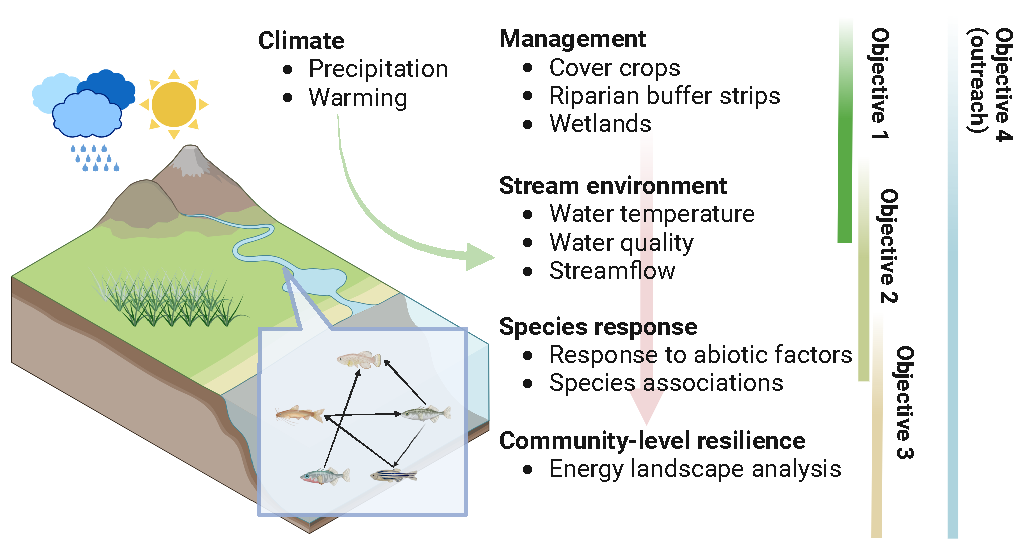
\includegraphics[scale=0.65]{output/fig_overview.pdf}
\caption{Project overview.
Objectives 1 -- 3 will be conducted in Year 1 -- 2.
Objective 4 will use the products from Objectives 1 -- 3 to communicate with stakeholders in Year 3.
Created with BioRender.com}
\label{fig:overview}
\end{SCfigure}

\section{Rationale \& Significance}

Our project will lead to substantial improvements in ecological health and resilience by providing novel tools to evaluate the effects of conservation practice portfolios on water quality and hence aquatic community resilience under current and future climate conditions.
As such, our proposal directly aligns with Program Area 4d, Priority (a): ``\textit{New approaches that substantially enhance ecosystem health and resilience, particularly in response to climate change, while increasing the output or value of multiple ecosystem services, compared to the current management system for the region.}''

First, we will develop \textbf{quantitative tools to evaluate \textit{aquatic ecosystem services at large spatial scales} that result from the implementation of cover crops, wetlands, and riparian buffers} -- water quality improvement, hydrological stabilization (\textit{Supporting Objective 1}), and the resulting improvement of ecological resilience in aquatic systems under climate change (\textit{Supporting Objectives 2 \& 3}).
Our modeling tools offer flexibility and can be adapted for the evaluation of other ecosystem services.
Moreover, we will enhance accessibility by creating a user-friendly programming package in R.
For instance, Terui has already initiated the development of the preliminary R package \url{snglmm}, which implements a geospatial model for \textit{Supporting Objective 1} (available at https://github.com/aterui/snglmm).
Consequently, our proposed project will significantly enhance our capacity to address a broad spectrum of water quality and ecological concerns in agroecosystems.

Second, we will expand upon an emerging multispecies modeling approach (an extension of Markov Networks) to concurrently estimate species responses to environmental changes and interspecific associations (\textit{Supporting Objective 2}).
Additionally, we will incorporate this advanced approach into ``Energy Landscape Analysis'' to empirically assess ecological resilience in the face of a changing climate (\textit{Supporting Objective 3}).
\textbf{Our innovative analysis enables us to forecast ecological resilience under changing climate conditions, utilizing existing spatial ecological data.}
While these quantitative tools will initially be applied to fish communities, they possess broad applicability across various ecosystem types (including terrestrial systems) and taxa.
Thus, our proposed work will serve as a foundational element for future research aimed at evaluating ecosystem health and resilience under a changing climate.

\textbf{Collectively, our quantitative framework will enable us to identify areas highly susceptible to climate change within the Midwest, leveraging existing data.} This invaluable information will guide spatial planning and prioritize conservation practices, ultimately leading to a significant enhancement of ecological resilience.

The research findings derived from these novel analytical methods will be seamlessly integrated into existing decision-support tools, which we have developed with input from stakeholders and key conservation partners (\textit{Supporting Objective 4}).
Our research findings will therefore reach beyond scientific communities, making a real difference in climate adaptation policies with a deeper understanding of how watershed conservation practices will improve the resilience of intensively managed landscapes.

\section{Approach}

\subsection{Supporting Objective 1}

\textbf{Specific Aim:} We will use extensive publicly available geospatial datasets and a novel geostatistical approach to identify relationships between existing implementations of conservation practices and surface water quality in streams and rivers across the entire Midwest (Figure \ref{fig:wq}).
Although current implementation rates of these promising conservation practices are low, there is sufficient spatial heterogeneity in implementation rates that we expect to detect a response in water quality. We will leverage a comprehensive water quality database, ``Water Quality Portal'' (WQP), developed by the Environmental Protection Agency and populated by water chemistry analysis of field samples collected from local, state, and federal agencies as a primary data source \citep{washington_dc_national_water_quality_monitoring_council_united_states_geological_survey_usgs_environmental_protection_agency_epa_water_2021}.

\begin{wrapfigure}{r}{0.4\textwidth}
    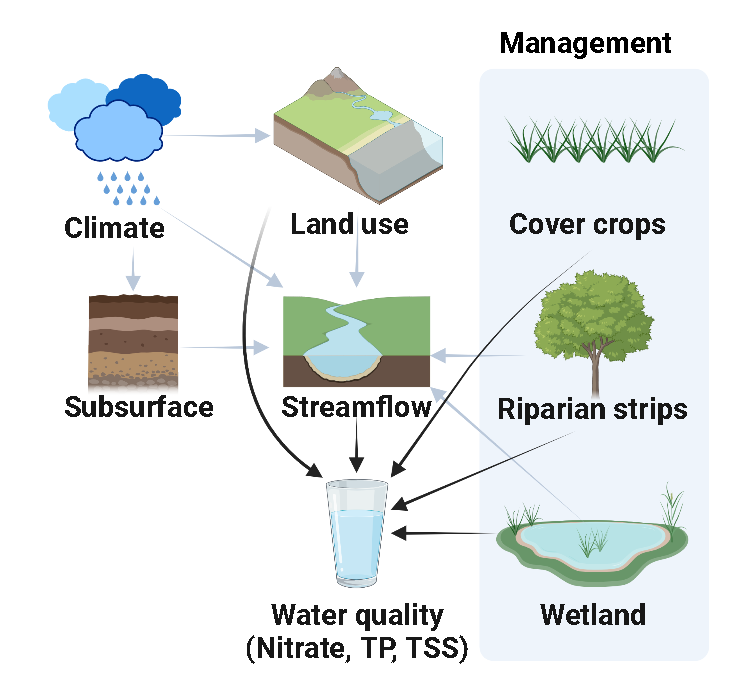
\includegraphics[scale=0.5]{output/fig_wq.pdf}
    \caption{Schematic diagram of factors affecting stream water quality. Black arrows indicate the pathways that will be quantified in this project. Gray arrows are the pathways that will not be incorporated into our predictive model but are accounted for in the global hydrodynamics models. Created with BioRender.com}
    \label{fig:wq}
\end{wrapfigure}

We will focus on three indicators of water quality, i.e, concentrations of \textit{nitrate}, \textit{total phosphorus} (TP), and \textit{total suspended solid} (TSS).
By considering surface water quality responses to conservation practices (cover crops, riparian buffer strips, and wetlands) across a large spatial area, we will also identify sub-regional differences in conservation action effectiveness.

\textbf{Methods -- Model Development}: Our baseline model is the relationship between stream chemistry (concentration $y_s$ [weight volume$^{-1}$]) and streamflow (discharge $F_s$) for site $s$:

\begin{equation}\label{eq:wq}
\log~y_s = \nu_0 + \nu_1 \log~F_s + \xi_{h(s)} + \varepsilon_s 
\end{equation}

where $\nu_0$ and $\nu_1$ are the parameters (the intercept and slope on a log scale) characterizing the power-law relationship between stream chemistry and discharge (Equation \ref{eq:wq} is $E(y_s) = e^{\nu_0}F_s^{\nu_1}$ on an ordinary scale), and $\varepsilon_s$ is the residual error term.
In this formulation, the intercept $\nu_0$ controls stream chemistry at the unit streamflow condition ($E(y_s) = e^{\nu_0}$ when $F_s = 1$ for a given discharge unit), thus governing the average stream chemistry (i.e., the geometric mean) at a given site.
In the meantime, the slope determines how stream chemistry scales with discharge. The parameter $\xi_{h(s)}$ is the random effect of the Hydrological Unit Code (HUC) defined by the USGS (HUC6 or HUC8; $h(s)$ is the HUC to which site $s$ belongs).
We will include this parameter to account for sub-regional variation.

We expect the chemistry-discharge relationship to be affected by seasonal and spatial factors.
To express the context dependency, we will assume that environmental contexts (details in the following paragraphs) change the intercept and slope:

\begin{equation}\label{eq:rwq}
\nu_{k, s} = (\nu'_k + \psi^{(k)}_{0,q(s)}) + \sum_d (\eta^{(k)}_d + \psi^{(k)}_{d,q(s)}) x_{d,s}
\end{equation}

In Equation \ref{eq:rwq}, the parameter $\nu_k'$ determines the baselines of the intercept ($k=0$) and slope ($k=1$) across sites, respectively.
The rest of Equation \ref{eq:rwq} captures how environmental contexts ($x_{d,s}$ is the value of $d$th spatial factor at site $s$) modulate the chemistry-discharge relationship through the regression parameter $\eta^{(k)}_d$ [$(k)$ distinguishes regression parameter of $d^{\text{th}}$ factor for $\nu_0$ and $\nu_1$].
The key environmental variables in this model are the type and extent of existing conservation practices, including cover crops (location and extent), riparian buffer strips (extent), and wetlands (type and extent).
Other environmental covariates include but are not limited to agricultural land use (crop type and extent, tile drainage density, animal operations) and topography.
Importantly, we will include the season-dependence parameter $\psi^{(k)}_{d,q(s)}$ ($d \in \{0, 1,...\}$), in which $q(s)$ represents the season of the observation date at site $s$ [spring (March-May), summer (July - Aug), fall (September - November), and winter (December - February)].
By including this term, the model can capture complex seasonal patterns of stream chemistry.
For example, cover crops might affect stream chemistry only during uncultivated seasons.
Seasonality $\psi^{(k)}_{d,q(s)}$ will be treated as random effects that follow a multivariate normal distribution because this expression will substantially decrease the number of parameters after marginalization.

To obtain environmental variables $x_{d,s}$, we will delineate subwatersheds for all sites with sufficient records of streamflow and water chemistry data using GIS (ArcGIS or directly with python code).
We expect this to be a set of $\sim$5000 sites. Streamflow monitoring data is available through US Geological Survey \citep{us_geological_survey_national_2001}.
Within each subwatershed, we will evaluate environmental characteristics as follows.

\textit{Conservation practices}.
\textit{Cover crops} -- We will characterize cover crops by the location and extent of cover crops, crop rotation, and any other data that is available regarding cover crop practice. 
The spatial distribution of cover crops is available as a geospatial dataset aggregated at the HUC8 level (OpTIS), \textcolor{red}{whose estimation accuracy was validated through ground truth surveys} \citep{the_nature_conservancy_optis_2023}.
Since OpTIS data is aggregated at the HUC8 level, which limits the quantity and resolution of the cover crop data, we will extend the analysis to the entire Midwest to secure sufficient variation in cover crops across sites.
\textit{Wetlands} -- We will characterize wetland type and extent from the National Wetlands Inventory (NWI) \citep{us_fish_and_wildlife_service_national_2024}.
The classification scheme within the NWI provides wetland aerial area, shape, and vegetation type.
In our geospatial analysis, we will determine the percent vegetation cover within wetlands, the ratio of wetland area to subwatershed area, and wetland interception of the contributing drainage area and wetland location with respect to the river network because our previous work, and that of others, suggests that these attributes are particularly important in controlling water quality downstream \citep{hansen_coupling_2016, cheng_maximizing_2020}.
\textit{Riparian buffer strips} -- Riparian buffer strip's width, extent, and vegetation type will be determined using geospatial analysis of the National Land Cover Database (NLCD; \citep{wickham_thematic_2021, wickham_thematic_2023}) developed by the USGS. Riparian buffers will be defined as non-agricultural land that is adjacent to a stream and located between an agricultural field and a stream and classified based on land use such as forested vs. grassland. Conservation practice location, subcategory, and extent will be verified for a subset of sites by comparing data products to an independent optical dataset (e.g., aerial imagery, Planet Labs satellite imagery).

\textit{Additional relevant geospatial data}.
\textit{Land use} -- We will evaluate land use, crop extent and type, soil type, animal operations, and tile drainage density. We will use NLCD for land use, USDA's Cropscape for crop type \citep{han_cropscape_2012}, either SSURGO or STATSGO for soil type \citep{us_department_of_agriculture_soil_2024, us_department_of_agriculture_us_2024}, Manuresheds for animal operations \citep{spiegal_manuresheds_2020}, and Agtile-US for tile drainage density \citep{valayamkunnath_mapping_2020}.
\textcolor{red}{These geospatial layers are peer-reviewed and quality-controlled, thus providing reliable input information for our statistical models.}
\textit{Topography} -- Topography (e.g., mean and SD elevation) will be obtained from digital elevation maps.

\textit{Model fitting}.
Our model can be developed as an ordinary hierarchical model, assuming statistical independence of residual errors as $\varepsilon_s \sim \mbox{Normal}(0, \sigma^2)$.
However, stream chemistry is spatially structured with strong upstream-downstream correlations \citep{peterson_patterns_2006, peterson_modelling_2013}.
If spatial autocorrelation is deemed important (highly likely), we will employ the spatial moving average approach developed for stream networks \citep{ver_hoef_spatial_2006}.
In principle, this method will take a weighted mean of residual errors given the relative spatial locations of sampling sites (e.g., upstream affects downstream but NOT \textit{vice versa}; the ``tail-up'' model \textit{sensu} \citep{peterson_modelling_2013}).
More specifically, we will decompose residual errors into non-spatial and spatial components:

\begin{equation}
\pmb{\varepsilon} = \pmb{\varepsilon_0} + \pmb{u},
\end{equation}

where $\pmb{\varepsilon_0}$ and $\pmb{u}$ denote non-spatial and spatial errors. We will assume a multi-variate normal distribution for $\pmb{u}$ as $\pmb{u} \sim \mbox{MVN}(0, \Sigma_{u})$, in which the variance-covariance matrix $\Sigma_{u}$ captures spatial non-independence between sampling sites.
We will start with a simple autocorrelation structure in the off-diagonal elements (e.g., exponential decay of upstream-downstream correlation) but will consider more complex autocorrelation structures if necessary (see \citep{ver_hoef_spatial_2006} for options).
This ``geospatial'' approach has two important benefits. First, it captures the fundamental nature of stream networks, i.e., upstream dictates downstream stream chemistry \citep{peterson_modelling_2013}.
Second, geospatial models are far more accurate in filling spatial gaps of observation \citep{ver_hoef_spatial_2006, peterson_mixed-model_2010, peterson_modelling_2013}.

\textbf{Methods -- Prediction}: While we will use this model to explore important controls of stream chemistry, this model will also allow us to predict water quality variables at fish survey sites in \textit{Supporting Objective 2}.
Once the model parameters are estimated, we will substitute values of environmental covariates $x_{d,s}$ with those measured at fish survey sites for prediction through regression-kriging \citep{hengl_about_2007}.
This predictive use is possible because all the environmental covariates in our model are GIS-derived.
The only exception is the streamflow; for this variable, we will use the estimates from the hydrodynamics model CaMa-Flood (see \textit{Supporting Objective 2} for details).

We will use space-for-time substitution to address the issue of spatial mismatch between water quality and fish survey sites.
In general, water chemistry data is collected at higher order streams than fish survey data due to limitations in sampling protocols and the original intended use for the separate datasets. 
For example, water chemistry monitoring sites are often collocated with streamflow monitoring sites (in order to calculate loads), whereas fish monitoring sites are typically lower-order streams to accommodate sampling protocols. 
In order to use the results of this analysis at fish survey sites, we need to understand how water chemistry scales with discharge ($\propto$ catchment size). 
Our model leverages the observed spatiotemporal variation in discharge to explicitly describe this relationship (Equation \ref{eq:wq}), thus providing robust predictions of stream chemistry at fish survey sites.

\textbf{Expected Results and Potential Pitfalls}: We expect that (i) nutrients and sediment in the stream water will increase with increasing discharge and agricultural land use; (ii) conservation practices will decrease the average and highest concentrations of nutrients and sediment and modify the slope of the power-law relationship between stream chemistry and discharge (Equation \ref{eq:wq}); and (iii) effects of conservation practices and land use are highly season dependent.

\begin{wrapfigure}{r}{0.45\textwidth}
    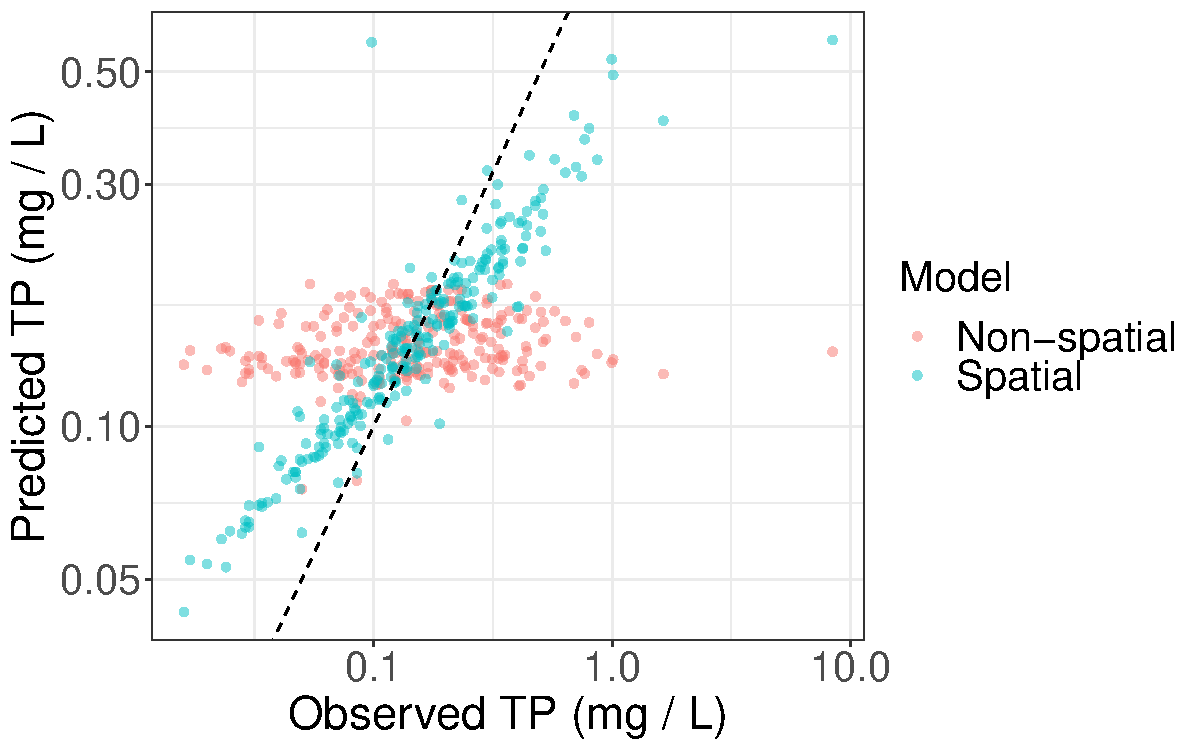
\includegraphics[scale=0.35]{output/fig_tpfit.pdf}
    \caption{Comparison of spatial and non-spatial models in the MRB (modeled variable: TP). The comparison of predicted (y-axis) and observed values (x-axis) proved the outstanding performance of the geospatial model (blue dots), surpassing that of the non-spatial model (red).}
    \label{fig:tpfit}
\end{wrapfigure}

Our model might face potential challenges when striving to provide accurate estimates of stream chemistry at fish survey sites. To verify the viability of our model, Terui has developed a novel R package named ``snglmm'' using the Template Model Builder (a development version available at \url{https://github.com/aterui/snglmm}). The Template Model Builder framework furnishes a C++ platform that facilitates the rapid and efficient fitting of intricate statistical models.
We fitted a simplified geospatial model (fixed effects: \% agriculture, \% wetland, and stream discharge) to monitoring data at 250 sites in the Minnesota River Basin (MRB). The model effectively captured significant impacts of land use and stream discharge on stream chemistry. Moreover, the integration of geospatial elements significantly enhanced the precision of model predictions (Figure \ref{fig:tpfit}) -- the predicted vs. observed values were aligned with the 1:1 line (broken line) that corresponds to the perfect prediction. Meanwhile, the prediction of the non-spatial model (simple regression) was far away from the 1:1 line, indicating the lack of predictive ability. As a result, we hold a high level of confidence in the reliability of our model.

One significant benefit of utilizing a statistical modeling approach is the ability to explicitly identify the underlying processes. In other words, we can gain insights into how conservation practices and alterations in land use impact water quality. Nevertheless, the presence of intricate, non-linear interactions can hold critical implications for ensuring accurate predictions. If we find that non-linear interactions are sufficiently large to mask the effect of conservation practice on water chemistry, we will adopt a machine-learning approach, such as a random forest model \citep{ryo_statistically_2017}, which is better suited for this type of data but does not uncover underlying process controls. 

\textcolor{red}{Various agencies populate WQP, potentially introducing data accuracy/consistency issues.
To mitigate this potential problem, we will diagnose the model residuals.
Any significant outliers (e.g., through the Grubbs test) given the environmental context at the site will undergo quality assurance checks.
We will remove the data point(s) from the analysis if it seems an error.
This strategy will give us the best estimate possible with the available information.}


\subsection{Supporting Objective 2}

\textbf{Specific Aim}: We will develop a multispecies statistical framework linking conservation practices, stream environments, and species occurrences with explicit consideration of species associations.
This analysis unveils (i) species association networks within metacommunities; and (ii) species-specific responses to conservation practices. 

We have assembled fish monitoring data across Minnesota \citep{minnesota_pollution_control_agency_development_2014}, Wisconsin \citep{wisconsin_department_of_natural_resources_guidelines_2018}, Iowa \citep{iowa_department_of_natural_resources_biological_2004}, and Illinois \citep{illinois_environmental_protection_agency_illinois_2014}.
This dataset contains the presence/absence of fish species at $>$ 4000 sites in the Upper Mississippi (Figure \ref{fig:fishmap}) and has been used in our previous research \citep{kim_metapopulation-level_2022, terui_emergent_2021}.
We will further extend this dataset to include additional data from the rest of the Midwestern states (Indiana, Kansas, Michigan, Missouri, Nebraska, North Dakota, Ohio, and South Dakota), which are also available from a public database \citep{hao_presence_2022}.
The observation period of the dataset is 1994 to 2019.
\textcolor{red}{Fish surveys were conducted using a standard sampling method (electrofishing), thus minimizing sampling biases across states.}

\begin{wrapfigure}{r}{0.35\textwidth}
    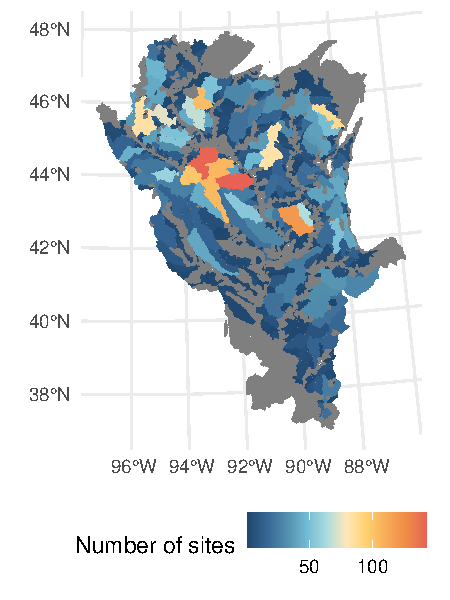
\includegraphics[scale=0.55]{output/fig_fishmap.pdf}
    \caption{Spatial mapping of the number of sampling sites. The number of sampling sites was colored by watershed (= metacommunity).}
    \label{fig:fishmap}
\end{wrapfigure}

\textbf{Methods -- Model Development}: We use conditional Markov Networks as a baseline of our statistical modeling (Figure \ref{fig:markovnet}).
Various scientific and engineering fields have used Markov Networks \citep{cheng_sparse_2014}.
Yet, this useful approach has rarely been applied to ecological data despite its enormous potential to capture complex ecological phenomena \citep{harris_inferring_2016, clark_unravelling_2018}.
This modeling approach is suitable for predicting complex community-level responses to climate change because it models the effects of species associations as predictors \citep{cheng_sparse_2014, harris_inferring_2016, clark_unravelling_2018}.
A potential alternative is the Joint Species Distribution Model (JSDM) \citep{warton_so_2015, ovaskainen_how_2017, pollock_understanding_2014}. However, while the JSDM approach is powerful, species associations are estimated as residual correlations instead of predictors \citep{ovaskainen_how_2017}.
For this reason, the model estimates cannot be used for future projections under environmental changes.

Here, we introduce the conditional Markov Network and subsequently extend it within a sparse-modeling framework.
The conditional Markov Network has the following model structure, focusing on one species at a time:

\begin{align}\label{eq:markovnet}
\begin{split}
&y_{si} \sim \mbox{Bernoulli}(p(y_{si}=1|y_{sj, j \ne i}))\\
&\log\left(\frac{p(y_{si}=1|y_{sj, j \ne i})}{1 - p(y_{si}=1|y_{sj, j \ne i})}\right) = \beta_{0,i} + \sum_k \beta_{k,i}x_{k,s} + \sum_{j, j \ne i} \gamma_{ij} y_{sj}
\end{split}
\end{align}

where $y_{si}$ is the presence/absence of fish species $i$ at site $s$, $x_{k,s}$ the value of $k^{\text{th}}$ environmental covariate, $\beta_{0,i}$ the species-specific intercept directly controlling the species prevalence, $\beta_{k,i}$ the effect of $k^{\text{th}}$ environmental covariate, and $\gamma_{ij}$ the strength of species association between species $i$ and $j$ ($\gamma_{ij} = \gamma_{ji}$).
In our project, we will group observation data by HUC8 watersheds and analyze them separately, as they represent an appropriate scale of metacommunities \citep{giam_environment_2016}.
HUC8 watersheds are small enough ($\sim$ 5000 km$^2$) to assume that fishes can disperse therein at a multi-generation time scale \citep{comte_fish_2018}.
This data grouping will help avoid spurious negative species associations due to geographic mismatch of species distributions.

While this model is designed to reveal species association networks, \textbf{it also estimates species-specific responses to environmental covariates $x_k$.}
Therefore, this approach allows us to identify species-specific sensitivity to water quality improvements by conservation practices.
We will consider the following environmental covariates $x_{k,s}$: \textit{streamflow variation}, \textit{water temperature}, \textit{nitrate}, \textit{TSS}, \textit{TP}, \textit{watershed area}, \textit{elevation}, \textit{riparian cover}, and \textit{spatial factors}.
Among these, climate (\textit{streamflow variation}, \textit{water temperature}) and water quality variables (\textit{nitrate}, \textit{TSS}, \textit{TP}) are the primary focus of this analysis.

\begin{wrapfigure}{r}{0.50\textwidth}
    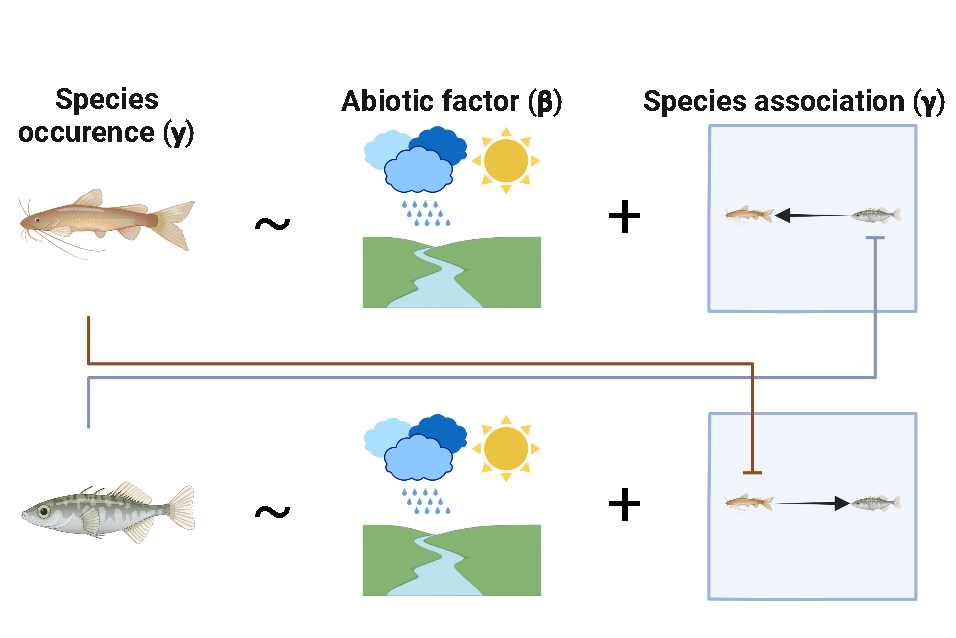
\includegraphics[scale=0.50]{output/fig_mn.pdf}
    \caption{Two-species example of Markov Network. Species occurrences are modeled \textit{jointly} as a function of abiotic factors and species associations - i.e., species occurrences are used both as a predictor and response in a single model. Created with BioRender.com}
    \label{fig:markovnet}
\end{wrapfigure}

\textit{Climate variables.} \textit{Streamflow variation} and \textit{water temperature} will be extracted from the global hydrodynamics models [streamflow, CaMa-Flood \citep{yamazaki_physically_2011}; water temperature, HEAT-LINK \citep{tokuda_development_2019}].
These hydrodynamics models have two key features.
First, model outputs are derived from the governing equations in physics with inputs of actual and future projections of meteorological data (e.g., radiation, specific humidity, cloud cover) and a land surface model (e.g., runoff, subsurface runoff, soil temperature).
Thus, the models account for critical processes controlling streamflow and water temperature (including groundwater processes).
Second, both models include inundation into floodplain areas during high flows. Through this process, the models account for streamflow stabilization and water temperature changes due to floodplains (including wetlands) in the landscape.
Currently, we have access to the global geospatial layer of streamflow and water temperature at a 25-km spatial resolution with daily estimates. However, Drs. Yamazaki and Tokuda, the developers of CaMa-Flood and HEAT-LINK models, have offered to provide model outputs with higher resolutions ($\sim$10 km) (see \textit{Letter of Support}).
We will perform a preliminary analysis with the geospatial layer at a 25-km resolution and will replace it with a higher resolution as it becomes available.

\textit{Streamflow variation} and \textit{water temperature} will be quantified as follows.
\textit{Streamflow variation} can be measured in many ways \citep{olden_redundancy_2003}.
Our measures of \textit{streamflow variation} may include, but not limited to, the interquartile range divided by the median, $\mbox{IQR} = \frac{Q_{95} - Q_{5}}{Q_{50}}$, where $Q_{u}$ is the $u^{\text{th}}$ percentile of the streamflow (discharge) in a given observation period.
$\mbox{IQR}$ represents the magnitude of extreme high and low flow conditions relative to the median; this measure is similar to the coefficient of variation but is robust to outliers (typical for streamflow data).
For $\mbox{IQR}$, we will group daily discharge data into 10-year bins to capture decadal trends and match them with the fish data (e.g., when a fish data point is observed in 1995, we will use $\mbox{IQR}$ from the 1991-2000 interval).
However, it is possible that organisms are adapted to seasonal cycles of streamflow at a given site. To consider this possibility, we will also calculate \textit{streamflow variation} as the deviation from monthly expectations.
This can be done by developing a simple linear model of log-transformed streamflow (log-transformed to account for non-normality) with the month as a predictor; the residual SD of the model represents the degree of deviation from monthly expectations.
For \textit{water temperature}, we will calculate the annual mean.
We will also calculate the summer mean (June - August) as a potential alternative to the annual mean because summer water temperature may exceed the physiological tolerance of some species.
Since metrics in the same category (\textit{streamflow variation} and \textit{water temperature}) will be highly correlated, we will perform a preliminary model selection for these variables and use one variable for each category.

\textit{Water quality.} Water quality variables (\textit{nitrate, TP, TSS}) will be estimated from the statistical model in \textit{Supporting Objective 1}, as direct measurements of these variables are rarely available at fish sampling sites.
The water quality model will allow us to impute missing values of these variables as we express the variables as a function of GIS-derived predictors.

\textit{Other factors.} The rest of the variables (\textit{watershed area}, \textit{elevation}, \textit{riparian cover}, and \textit{spatial factors}) are control factors that will be obtained from GIS.
We will include these variables because they are known to control stream size, substrate coarseness, current velocity, and microhabitat availability \citep{altermatt_diversity_2013, finlay_stream_2011, terui_three_2016}.
Although our data set of fish communities does not contain detailed environmental variables, the inclusion of these environmental variables will allow the model to capture local variations in environmental conditions.
\textit{Spatial factors} are the variables that account for spatial ecological processes. For example, they may include the effect of dispersal.
We will use the network centrality measures of the stream networks to approximate spatial effects.
Network centrality measures, which can be calculated solely from stream network structure, have been used as a proxy for connectivity \citep{altermatt_river_2013, watson_identifying_2011}.
Although there are several measures of network centrality, we will use ``betweenness'' or ``eigenvalue'' centrality as our preliminary analysis indicated these measures are clearly correlated with fish occurrences. By accounting for this effect, we can indirectly incorporate the influence of dispersal in ecological forecasting (see \textit{Supporting Objective 3}).

\textit{Model fitting.} Conditional Markov Networks can estimate species associations.
However, fitting the model to the data is challenging because there are many parameters of species associations $\gamma_{ij}$. We need to estimate $\frac{I(I-1)}{2}$ parameters ($I$ is the number of species) to build a complete network of species associations, and this number rises exponentially as the number of species increases.
We address this statistical issue by introducing sparse modeling to Markov Networks \citep{cheng_sparse_2014}.
Sparse modeling is a statistical technique to reduce the complexity of a model by inducing zeros to some of the statistical parameters \citep{cheng_sparse_2014, lunn_bugs_2012, mutshinda_what_2009}.
The sparse modeling can be implemented in R using the `glmnet' package and has been proven to provide reliable estimates of species associations \citep{clark_unravelling_2018}. 

\textbf{Expected Results and Potential Pitfalls}: The proposed modeling framework can infer important ecological processes from the presence/absence data, representing a promising tool for climate change research in managed landscapes.
Therefore, we expect this modeling framework will advance the field significantly.
We expect the following:
(i) Conservation practices that effectively reduce TSS will most benefit fish populations because sedimentation is a leading cause of fish declines, particularly those occupying higher trophic positions \citep{kemp_impacts_2011}; and 
(ii) Substantial reduction of stream nutrients may decrease the occurrence of primary consumers (detritivore/algivore) as reduced nutrients may limit food availability for those fish species. 

There are several caveats that need to be addressed.
First, there is no guarantee that model estimates converge.
To address this risk, we performed a preliminary analysis using fish community data at the MRB (25 species at 435 sites).
The sparse modeling approach identified key associations among 25 fish species within the watershed, unveiling the predominance of positive species associations in this system (links in Figure \ref{fig:fishnet}).
Thus, our modeling approach is feasible and robust.
Given the results from the MRB, we anticipate the significant role of species associations in driving the ecological resilience of fish communities under climate change.

\begin{wrapfigure}{r}{0.3\textwidth}
    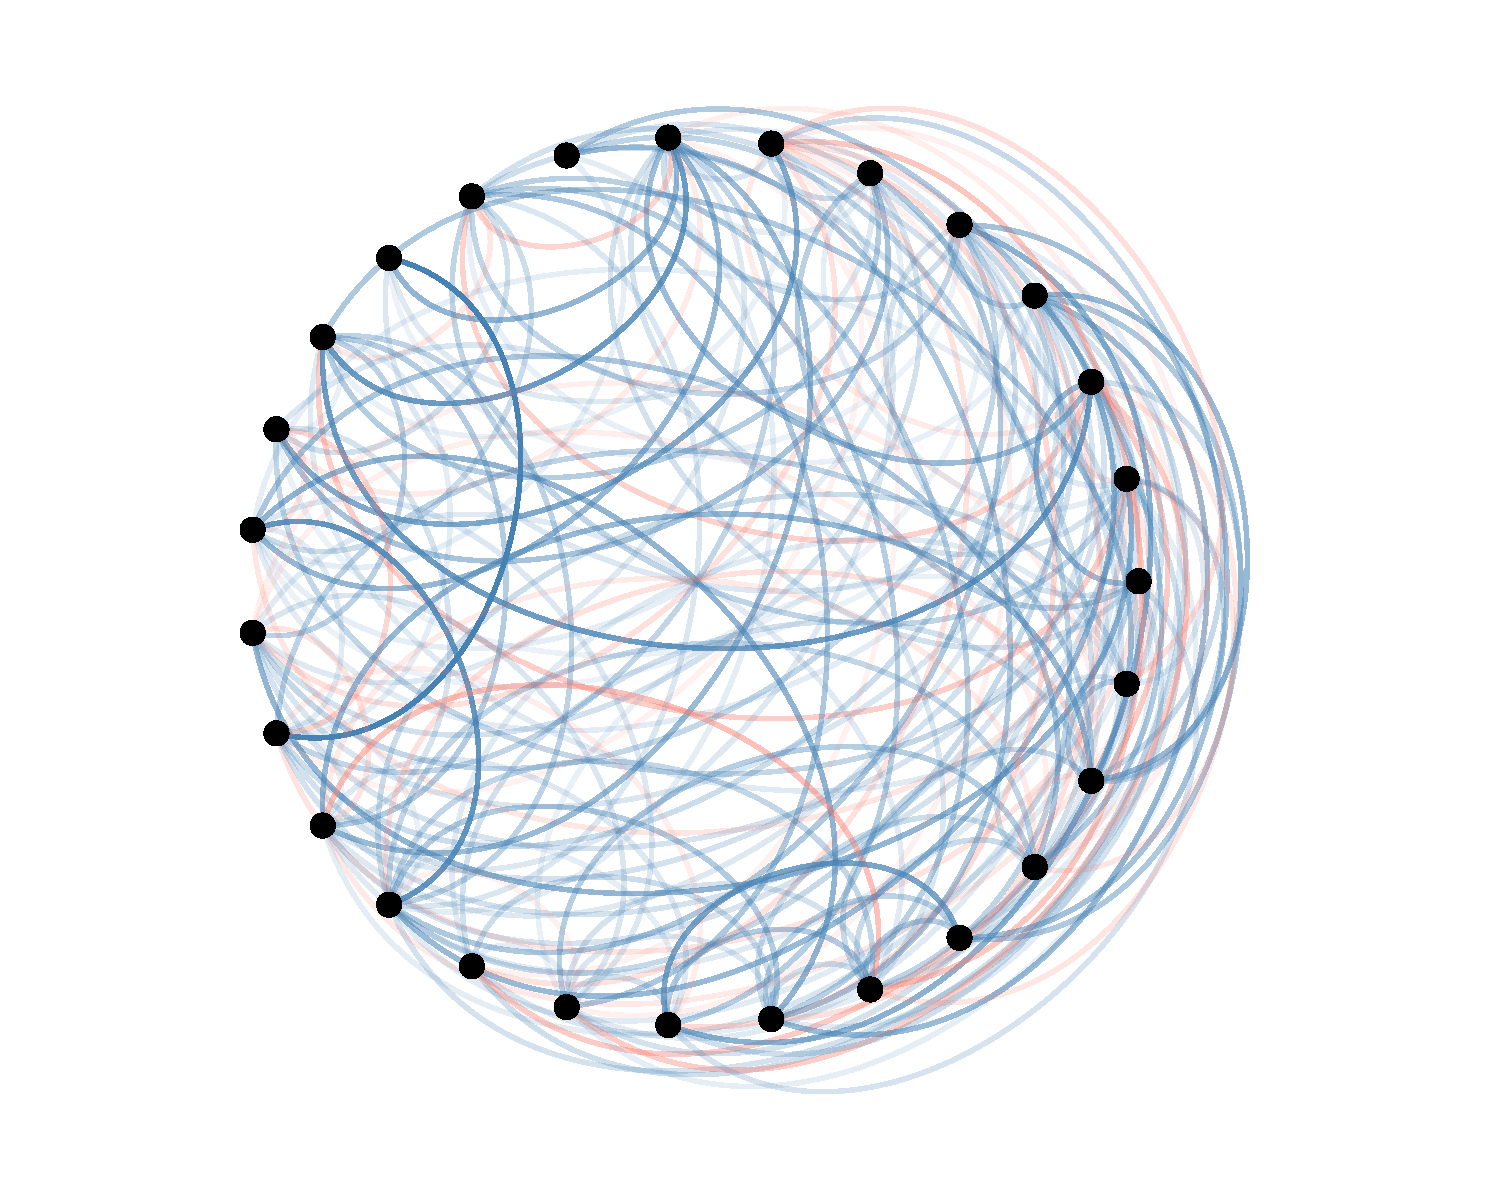
\includegraphics[scale=0.2]{output/fig_fish_network.pdf}
    \caption{Markov Network Analysis revealed complex species associations in the Minnesota River Basin. Each node represents fish species, and links connecting nodes denote species associations. Link transparency is proportional to the strength of species association, and color indicates positive (blue) and negative (red) associations.}
    \label{fig:fishnet}
\end{wrapfigure}

This preliminary analysis has also yielded valuable insights into the potential response of various species to conservation practices.
We incorporated agricultural land usage as one of the key environmental variables, and the specific reactions of different species were correlated with their ecological characteristics.
Within the Fish Traits Database's comprehensive range of ecological traits \citep{frimpong_fish_2009}, we identified that trophic status (differentiating between predators and primary consumers) and body size stand out as significant predictors of fish responsiveness to increased agricultural land use.
Larger-bodied fish occupying higher trophic positions (e.g., northern pike, walleye) display a greater susceptibility to the impacts of intensified agricultural land use. 
Consequently, we anticipate that species with such traits stand to gain more from conservation practices.

Second, our fish dataset is heterogeneous in the sampling year and data source (e.g., state) as these data were assembled from multiple states.
This complexity could bias parameter estimates.
If this heterogeneity is deemed important, we will address it by extending the Markov Network to include covariates of sampling year and data source ID.
This is just one \textit{example} of the statistical adjustments we can make.
This modeling framework is very flexible and robust to common problems in large ecological datasets.

\textcolor{red}{Lastly, the lack of conservation effects on fish species could be attributable to insufficient sample size (the number of sites).
To address this concern, we will use simulated data generated from process models with known parameters.
The comparison of statistical estimates and the true parameter values will allow us to assess the appropriate sample size given the number of predictors used.
In doing so, we can assess and minimize the risk of Type II error (false rejection of conservation effects).}

\subsection{Supporting Objective 3}

\textbf{Specific Aim}: We will assess (i) how agricultural land use and climate change impact the ecological resilience of stream fish communities through stream environment changes; and (ii) how conservation practices offset the potential impacts of agricultural land use and climate change.
We tackle these questions with the following methods.

\textbf{Methods -- Resilience Metrics}: We will employ a novel analytical technique known as ``Energy Landscape Analysis'' \citep{suzuki_energy_2021}. Originally developed in the field of statistical physics, this method quantifies the energy associated with a particular community structure ($E$), which is defined as follows:

\begin{align}\label{eq:energy}
E = -(\sum_i \beta_{0,i} y_i + \sum_i \sum_k \beta_{k,i} x_{k} y_i + \sum_i \sum_j \gamma_{ij} y_i y_j / 2)
\end{align}

\begin{wrapfigure}{r}{0.375\textwidth}
    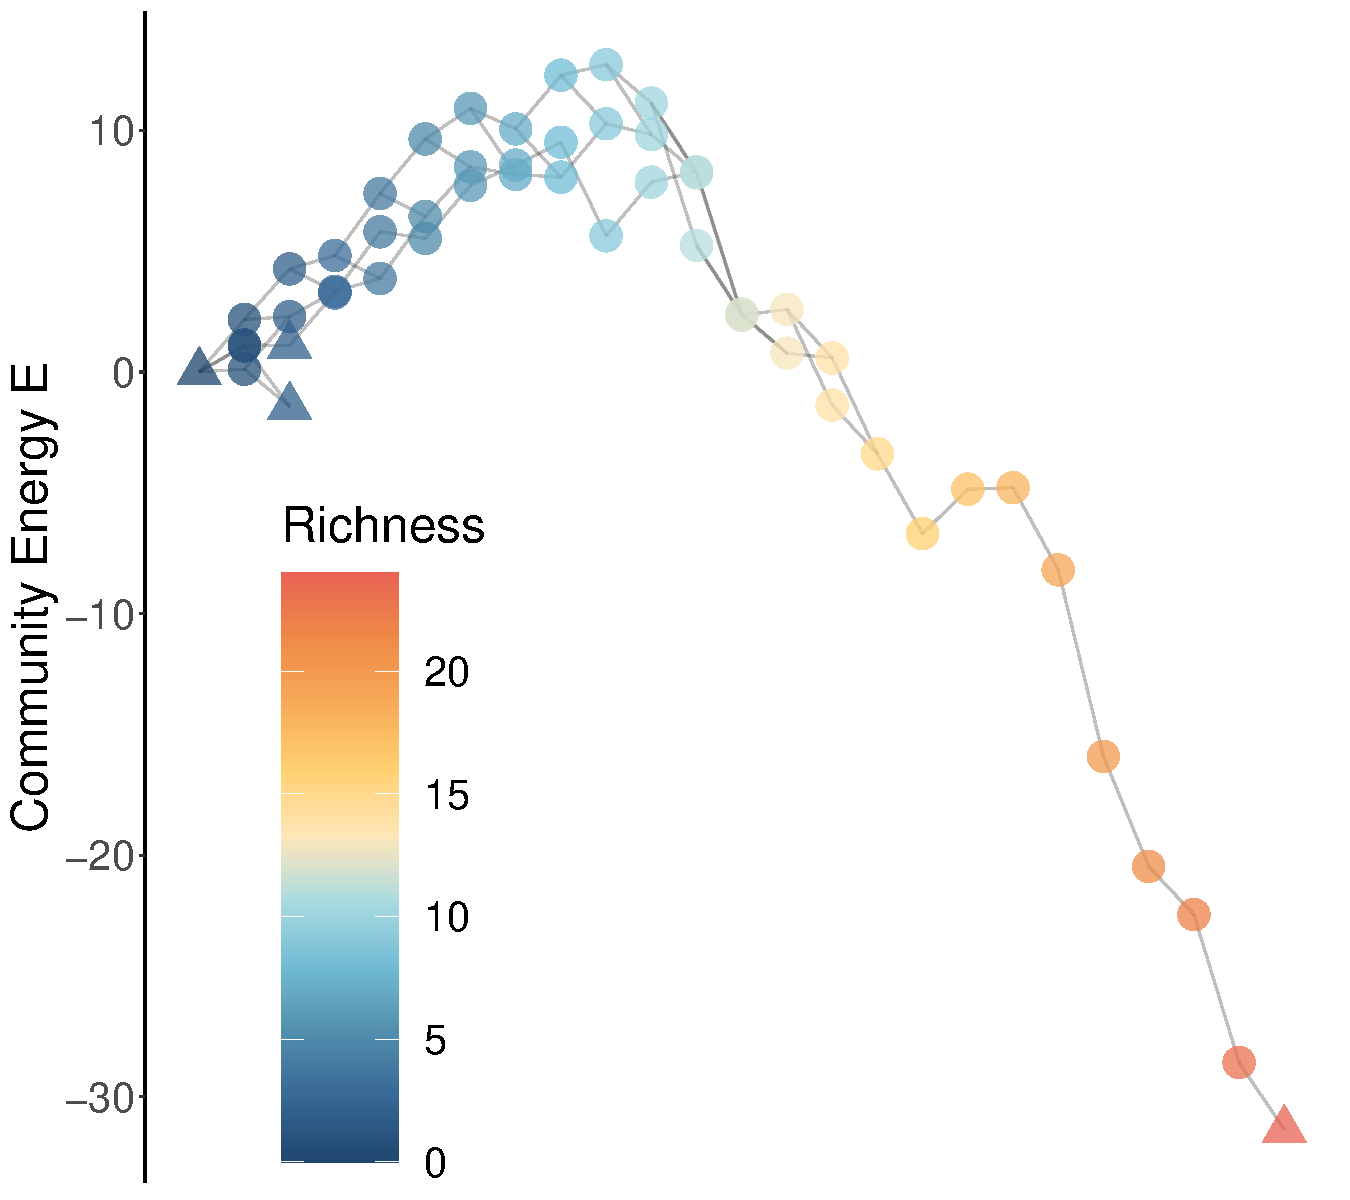
\includegraphics[scale=0.275]{output/fig_ela_mrb.pdf}
    \caption{Energy landscape of fish communities at the Minnesota River Basin, which was constructed based on the preliminary analysis in \textit{Supporting Objective 2} (in this example, 80 \% agricultural land use was used to construct). Each node represents a distinct community composition and links denote possible transitions among them (see Box 1 for details). Small and large circles show transient and stable community states (stable states are the local minima in the energy landscape). Each community state is colored in proportion to species richness (0--25). Only the shortest paths connecting stable states are shown for a visual purpose.}
    \label{fig:ela}
\end{wrapfigure}

where $y_i$ ($y_j$) represents the presence/absence of species $i$ ($j$), $x_k$ is the $k^{\text{th}}$ abiotic predictor, and $\beta_{0,i}$, $\beta_{k,i}$ and $\gamma_{ij}$ are the parameters estimated in the Markov Network Analysis (Equation \ref{eq:markovnet}).
This analysis generates a mathematical representation of the community energy landscape, in which we can identify energy ``basins'' and ``ridges'' of community compositions (Figure \ref{fig:ela}; see Box 1 for details).
The lowest points of basins correspond to local energy minima, indicating that community compositions tend to gravitate towards them.
Thus, community compositions representing the local energy minima behave like ``stable states'' in theoretical community ecology.
On the other hand, ridges represent critical junctures where the direction of community shifts becomes highly uncertain, resembling ``tipping points.''

Here, we define ecological resilience $\phi$ as the ``roughness'' of the energy landscape because the likelihood of moving away from one stable state to another is dependent on the depth of local minima \citep{suzuki_energy_2021}.
In practice, we will measure the average height of energy barriers between local minima \citep{suzuki_energy_2021}:

\begin{align}\label{eq:phi}
\phi = \frac{\sum_i \sum_{j, j \ne i} H_{ij}}{N_{barrier}}
\end{align}\label{eq:phi}

where $H_{ij}$ is the height of an energy barrier separating local minima $i$ and $j$, and $N_{barrier}$ is the number of energy barriers in the energy landscape.
The low $\phi$ indicates the flatter energy landscape, implying that small perturbations can cause drastic shifts in community structure.
In contrast, the high $\phi$ indicates the prevalence of deep basins, which require strong external force to move from one stable state to another.

\textbf{Importantly, our metric of ecological resilience has a clear connection to climate (water temperature, discharge variation), conservation practices, and species associations} because community energy $E$ is defined as a function of those variables.
In particular, this formulation allows us to assess how environmental changes will increase/decrease the ecological resilience $\phi$ through changes in the energy landscape (Figure \ref{fig:ela}). 

\textbf{Methods -- Drivers of Resilience}: Using the resilience metric $\phi$, we aim to address the following questions:

\begin{enumerate}
    \item \textbf{How does agricultural land use impact the ecological resilience of aquatic communities?}
    To investigate this, we will produce energy landscapes with different levels of agricultural land use using equation \ref{eq:energy}.
    This allows us to quantify the ecological resilience $\phi$ at each level of agricultural land use. In particular, we will focus on the mechanistic linkages through stream chemistry (nitrate, TP, and TSS).
    This is possible because we will establish the statistical relationship between agricultural land use and stream chemistry values in \textit{Supporting Objective 1}.
    \item \textbf{How does climate change, characterized by warming water temperatures and increased discharge variation, affect the ecological resilience of aquatic communities?}
    To investigate this, we will utilize future climate projections provided by the CaMa-Flood and HEAT-LINK models at a resolution of approximately 10 km (see \textit{Letter of Support}).
    By substituting climate variables with projected values ($x$ in Equation \ref{eq:energy}), we can forecast ecological resilience under different climate change scenarios (RCP 2.6, 4.5, 6.0, 8.5).
    This approach will enable us to identify the areas that are susceptible to climate change.
    \item \textbf{How can conservation practices mitigate the anticipated effects of climate change on ecological resilience?}
    Through \textit{Supporting Objectives 1-2}, we will establish connections between conservation practices, stream water quality, and fish species response.
    This modeling effort enables us to project how hypothetical changes in conservation practices will offset the impacts of climate change on ecological resilience $\phi$.
    Specifically, we will hypothetically increase wetlands, riparian buffers, and cover crops under climate change scenarios.
    The predicted $\phi$ values will be compared with those that are derived without any changes in conservation practices (i.e., $\phi$ values predicted in Question 2).
    This analysis will allow us to visualize the potential benefits of conservation practices under climate change.
\end{enumerate}

\textbf{Expected Results and Potential Pitfalls}: We expect: (i) ecological resilience will decrease with the intensification of agricultural land use; (ii) climate change will compromise the ecological resilience of aquatic communities; (iii) conservation practices will offset the potential impact of climate change on the ecological resilience.

Our preliminary analysis at the MRB confirmed that ecological resilience decreased with agriculture intensification -- the energy landscape became ``flatter'' as agricultural land use increased, inflating the risk of abrupt shift from species-rich (the local minimum on the right, Figure \ref{fig:ela}) to species-poor communities (the local minima on the left, Figure \ref{fig:ela}).
We expect that conservation practices have the potential to mitigate this adverse effect of agriculture and its potential synergies with climate change.
Yet, it is conceivable that conservation practices have little influence on ecological resilience, given the complexity of species associations.
Even so, our analysis will still provide useful management implications as it suggests that distinct approaches are needed to achieve water quality improvement and biodiversity conservation.

Our research outputs will offer valuable and novel insights to conservation practitioners for the following reasons.
First, our analysis effectively pinpoints the areas in the Midwest that are most susceptible to the impacts of climate change. This information can serve as a guiding tool for prioritizing spatial conservation efforts and making prudent decisions regarding the allocation of limited conservation funds.
Second, our results will illuminate significant disparities, if any, among various conservation practices in their ability to enhance ecological resilience. This information will help in identifying potential trade-offs when investing in distinct conservation strategies, making it vital for future economic analyses.
Lastly, our analytical approach is exceptionally versatile and can be applied to diverse agroecosystems and taxa.
Consequently, our modeling methodology holds immense potential to enhance our capacity to assess and subsequently enhance ecological resilience in the face of projected climate change.

\begin{tcolorbox}[parbox=false, breakable]
    Box 1: Energy Landscape Analysis
    \tcblower
    In the context of community ecology, the energy landscape represents a network in which each node corresponds to a unique community composition.
    The links between nodes indicate transitions between these compositions, and each transition is associated with a specific change in the presence/absence of a single species.

    This analysis assigns an ``energy'' value to each composition such that low energy values indicate a higher probability of occurrence.
    The probability of observing a community composition $O^{(p)}$ is calculated using the equation $\Pr(O^{(p)}) = \exp(-E^{(p)})/Z$
    
    Here, $O^{(p)}$ represents the community composition $p$, which is indicated by a binary permutation of $S$ species in a watershed.
    This results in $2^S$ possible community compositions. The normalization constant $Z$ is calculated as the sum of the exponential of the negative energy values for all compositions ($Z = \sum_p^{2^S} \exp(-E^{(p)})$).
    The community energy, denoted as $E$, can be defined using parameters estimated in the Markov Network Analysis (Equation \ref{eq:energy}).
    
    If deterministic, the transitions between community compositions follow the energy gaps between neighboring nodes.
    Consequently, communities tend to gravitate toward the lowest points of attraction basins (local energy minima), which serve as empirical proxies of ``stable states.''
\end{tcolorbox}

\subsection{Supporting Objective 4}

\textbf{Specific Aim}: The Nature Conservancy (TNC) has an extensive network of conservation practitioners who collaborate with agricultural producers, local, state, and federal agencies, supply chain companies, and agricultural retailers across the Midwestern US.
Drawing upon this well-established network in the region, we aim to integrate the results from \textit{Supporting Objectives 1--3} into a decision support tool that was designed and developed using direct stakeholder input as part of the USDA's Upper Mississippi Conservation Effects Assessment Program-Wildlife (CEAP-Wildlife; Hansen, Piazza co-PIs).
Because the CEAP-Wildlife effort took a first step to identify the effects of agricultural BMPs (Best Management Practices) on aquatic biota and create a product to support practical agricultural conservation decision-making, building on this tool will ensure continued buy-in from regional partners, minimize ``tool fatigue,'' and improve an existing user-driven tool in a way that directly benefits conservation.
Specifically, understanding the influence of climate change on freshwater biodiversity and water quality responses to agricultural conservation practices has been identified by stakeholders as a critical need that the CEAP tool does not yet address. The specific aim of \textit{Supporting Objective 4} is to fill this need.

\textbf{Methods -- Network Engagement}: Through the CEAP-Wildlife effort, TNC is tapping into its extensive network of key conservation practitioners and partners to model the effects of conservation BMPs on water quality and aquatic health in the upper Mississippi River Basin and engage with people on the ground to scale-up conservation across the agricultural landscape.
In our communications, we have discovered that stakeholders in our region are deeply concerned about the impacts of climate change.
We have specifically identified a critical knowledge gap concerning how conservation practices can effectively enhance the ecological resilience of managed landscapes in the face of climate challenges.
Using this same established network, we will elicit input and feedback on the practical application of the existing CEAP tool to determine how to effectively integrate the results of \textit{Supporting Objectives 1--3} (see details below) in a way that best meets stakeholder needs and increases the scope and scale of conservation BMPs across the agricultural Midwest. 

Additionally, we recognize the pivotal role of key influencers in shaping perspectives and decisions.
To actively involve them, we will maintain regular communication, providing timely research updates and keeping them well-informed about the latest developments in the field.
Furthermore, we will seek their invaluable feedback, understanding their needs and preferences, to ensure our initiatives align seamlessly with their aspirations.

\textbf{Methods -- Tool Development}: We will produce comprehensive spatial data that depict water quality, biodiversity, and ecological resilience across the region, under four climate change scenarios previously identified (RCP 2.6, 4.5, 6.0, and 8.5).
These data will be the outputs from \textit{Supporting Objectives 1--3} (refer to Figure \ref{fig:overview}).
For each river segment, we will assign predicted values (water quality, local biodiversity \& resilience) with proportional coloration, considering segments between confluences.
To provide a long-term perspective, we intend to generate spatial data at 10-year intervals, projecting up to approximately 100 years into the future, with the baseline set in 2020 (note that the latest fish data available is from 2019).

The CEAP-Wildlife tool currently allows users to determine how well a given amount and placement of conservation actions will achieve nutrient and sediment reduction and aquatic biodiversity conservation goals within the upper Mississippi River basin.
With the addition of climate change scenarios, we will be able to model the need for supplementary agricultural conservation practices to achieve these goals in response to the effects of changing temperature and rainfall patterns.
These data will be directly integrated into the already existing watershed boundary datasets that were created for the CEAP-Wildlife tool.
Within the enhanced CEAP-Wildlife decision support platform, these integrated datasets will be visualized at various scales from stream reach to basin scale.
We will implement functionality that will allow users to explore and simulate the adoption of agricultural conservation practices within the region at current conditions and four climate change scenarios.
This will help users understand the potential benefits of conservation efforts in enhancing the ecological resilience of impacted watersheds.

Leveraging our recent work on decision support systems at large scales and specifically within the upper Mississippi River basin, the PIs are uniquely positioned to frame this work coherently within the existing regional network of stakeholders and practitioners and to deliver agricultural conservation information to a targeted audience for the purpose of large-scale practice adoption.
Our efforts will harness the collective knowledge and efforts from diverse research projects, fostering broader community engagement.

% \textbf{Expected Synergies.} We anticipate additional synergies arising from various collaborations.
% The recently established Midwest Climate Adaptation Science Center (CASC), with its leadership based at the University of Minnesota, will provide crucial resources for public engagement.
% Notably, Finlay is a fellow at the Institute on the Environment, which serves as the central hub for the Midwest CASC.
% This affiliation will further enhance our capabilities for engaging with the public and stakeholders.

% Additionally, Dolph and Finlay, as co-PIs, have secured support from the EPA for a collaborative project.
% This joint effort aims to compile and analyze river biological data in the Mississippi River Basin, subsequently integrating it into economic models to develop innovative methods for water quality valuation.
% Through these various opportunities and partnerships, we actively seek synergistic activities that will amplify community engagement across the region.

% By seamlessly integrating research outputs and engaging key stakeholders, we can effectively address the challenges posed by climate change and foster a sustainable and resilient future for the study region.

\newpage

\fancyhead[L]{Bibliography \& References Cited}
\renewcommand{\bibsection}{\section*{Bibliography \& References Cited}}
\bibliography{references}
\end{document}
